% ==============================================================================
% PG - Nome do Aluno
% Capítulo 3 - Contribuição
% ==============================================================================
\chapter{Análise e Projeto}
\label{sec-contribuicao}

% Este capítulo deve apresentar a principal contribuição do trabalho. Caso o aluno e orientador desejem, o título do capítulo pode ser alterado para referenciar diretamente a contribuição (por exemplo, PIS: Plataforma para Integração de Serviços; Um Sistema para Controle de Processos da UFES, Solução de Otimização para Carregamento de Contêineres; etc.)

% O capítulo deve ser estruturado em seções de forma a apresentar de forma clara e com todas as informações necessárias, a contribuição do trabalho. Por exemplo, caso a contribuição produzida seja um sistema de informação, espera-se que sejam apresentados seus requisitos, funcionalidades, modelos (p.ex., modelo estrutural, modelo da arquitetura, etc.) e telas do sistema. Caso seja uma plataforma, espera-se que a plataforma como um todo seja apresentada e que seus componentes sejam descritos sejam apropriadamente.

Este capítulo tem o propósito de detalhar o escopo do jogo Super Labes World, aplicando os conceitos de engenharia de software para então identificar seus requisitos e finalmente criar o diagramas de classe. Na seção \ref{sec:descricao-do-cenario} fazemos uma breve explicação do cenário que foi incentivo para a criação desse trabalho, a seção \ref{sec:escopo} descreve o intuito desse trabalho, na seção \ref{sec:jogo} é descrito o design do jogo e também os possíveis usuários desse software, na seção \ref{sec:requisitos-do-jogo} é feito o levantamento de requisitos do jogo e com tudo isso em mãos, foi possível criar o diagrama de classes seção \ref{sec:diagrama-de-classes}.


\section{Descrição do Cenário}
\label{sec:descricao-do-cenario}
Alice, uma estudante hipotética recém-chegada ao curso de ciência da computação na UFES, sonhava em participar de projetos práticos que envolvessem programação e inovação e que fizessem diferença na sociedade. Com isso em mente, ela decide se candidatar ao LabES, um laboratório de extensão da UFES. Pouco tempo após preencher o formulário no site ela é contactada pela equipe responsável pelo embarque e rapidamente entra em um dos projetos.

Ao começar no projeto ela percebe que é a mais nova dentre os membros e não entende alguns termos e ferramentas utilizados entre eles; ela também percebe que há um grande volume de informações iniciais sobre o laboratório e também sobre o projeto. Pat, a professora coordenadora, Bob, membro sênior, junto aos demais estudantes do projeto, estão repletos de atividades e não conseguem dar atenção inicial necessária para ajudar Alice. Contudo, Alice é uma estudante dedicada e persegue os seus objetivos; diante dos desafios, ela elaborou um plano de estudos e o aplicava durante as noites. Após semanas de estudos, Alice começou a dar bons resultados no projeto.

Situações similares a esta ocorrem diariamente em vários laboratórios da UFES. Alguns estudantes, como Alice, conseguem se organizar de forma autônoma e, depois de algum tempo, passam a produzir para o projeto. Outros estudantes não têm a mesma resiliência e persistência de Alice e acabam desistindo no meio do caminho; ou então levam um tempo demasiado para conseguirem produzir, o que pode gerar uma certa desmotivação. Trata-se de um problema complexo, no qual que não existe um único culpado e nem um único ponto a ser resolvido. 

\section{Escopo}
\label{sec:escopo}
Diante da situação descrita na seção \ref{sec:descricao-do-cenario}, surge a ideia de criar o \textit{Super Labes World}, um jogo RPG \textit{desktop} desenvolvido com o intuito de ser uma ferramenta lúdica e didática, que possa ser utilizada para apoiar os estudantes em processos de ``embarque'' em laboratórios. A ideia é que o jogo possa ser usado para testar, reforçar e adquirir novos conhecimentos. Em sua versão inicial, o jogo foca em estudantes do LabES e, portanto, considera questões inerentes ao laboratório; porém, futuramente, com as devidas alterações/extensões, o jogo pode ser considerado para outros laboratórios e áreas da UFES.

\section{O Jogo}
\label{sec:jogo}

O jogo começa com o personagem acordando em sua casa e lembrando que precisa realizar um teste para entrar no projeto SigAMAES do LabES. Após este primeiro momento, a ambientação do jogo se passa na UFES. Durante a exploração inicial e interação com personagens, o jogador é dirigido ao prédio CT7, onde estão localizados o laboratório e os professores e, assim, pode começar a ``batalhar'' com alguns dos professores, que são os chefes a serem vencidos. A batalha é no estilo perguntas e respostas sendo que o jogador tem quatro opções para escolher. O tema das questões depende de cada professor, que são mestres em disciplinas específicas. Alguns exemplos de conteúdo de batalhas:

\begin{itemize}
    \item \textbf{Professor Vitor: }contém perguntas relacionadas a área de programação em java e conceitos de \textit{docker};
    \item \textbf{Professora Monalessa: }contém questões relacionadas a git, gitlab e gitflow;
    \item \textbf{Professora Patrícia: } contém as questões sobre a metodologia do LabES.
\end{itemize}

Ao final da batalha, caso o jogador vença, o professor entrega sua chave, representando a sua aprovação nesta disciplina. Somando as três chaves, o jogador pode finalmente ter acesso ao LabES. Caso o jogador erre mais do que 30\% das perguntas, a batalha é finalizada e o professor o instrui a utilizar o \textit{computador}. O \textit{computador} é uma mecânica do jogo que pode ser acessada a partir dos mapas ``sala do professor'' e ``labgrad'' e contém os \textit{links} para materiais de estudos abordados nas questões que o jogador errou. Ao clicar nesse \textit{link}, o jogador será redirecionado a esse conteúdo para estudar, aprender e tentar passar de nível novamente.

\subsection{Usuários}
\label{sec:usuarios}
O Super Labes World é uma versão inicial de um jogo que tem potencial de ser extensível. Foram identificados três potenciais usuários deste trabalho:

\begin{enumerate}
    \item \textbf{Estudantes da UFES que desejam iniciar no LabES:} O principal usuário do Super Labes World são estudantes da UFES que desejam iniciar ou são iniciantes no LabES. Toda a história, músicas, efeitos sonoros, interface, itens, questões, diálogos de personagens e personagens foram criados com isso em mente, de forma que o jogador possa se identificar e manter-se engajado no \textit{game}. 
    \item \textbf{Professores:} Um outro possível usuário do jogo são professores que podem alterar as perguntas e recriar o jogo, para diferentes propósitos. 
    \item \textbf{Estudantes de computação:} O jogo pode ser interessante para qualquer estudante de computação, uma vez que trata de questões da área.
\end{enumerate}

\section{Requisitos do Jogo}
\label{sec:requisitos-do-jogo}
A partir do escopo do projeto apresentado na seção \ref{sec:escopo}, os requisitos identificados foram organizados em tabelas. A tabela \ref{tbl-requisitos-funcionais} apresentada os requisitos funcionais e, na tabela \ref{tbl-requisitos-de-dominio}, os requisitos de domínio.

Um dos principais indicadores de sucesso de um sistema de software é o nível de atendimento aos requisitos para os quais foi projetado. Os requisitos de um sistema de software abrangem as descrições das funcionalidades que o sistema deve prover, e das restrições que devem devem ser atendidas. Em essência, os requisitos definem o que o sistema deve fazer e as
circunstâncias sob as quais deve operar. \cite{sommervilleengenharia}

Requisitos funcionais definem os serviços e tarefas que o sistema deve prover. Eles descrevem as funcionalidades específicas do software. Requisitos de domínio (ou regras de negócio) são provenientes do domínio de aplicação do sistema e expressam características e restrições próprias desse contexto. Eles são baseados no negócio que o sistema visa atender, podendo limitar requisitos funcionais já definidos ou estabelecer como cálculos específicos devem ser realizados, refletindo fundamentos do domínio de aplicação. \cite{sommervilleengenharia}.

 
\begin{table}[h!]
	\caption{Tabela de requisitos funcionais do Super Labes World.}
	\label{tbl-requisitos-funcionais}
	\centering
	\renewcommand{\arraystretch}{2}
	\begin{small}
		\begin{tabular}{ | p{20mm} | p{102mm} | p{20mm} |}\hline \rowcolor{MidnightBlue}
			\centering{\textbf{Id}} & \textbf{Descrição} & \textbf{Relação} \\\hline		
                \centering{RF1} & O jogo deve ser controlado pelo teclado &  \\\hline
			\centering{RF2} & O jogo deve ter um menu inicial. &  \\\hline
                \centering{RF3} & O jogo deve ter uma interface que mostre os controles do jogo. & RF2 \\\hline
			\centering{RF4} & O jogo deve ter uma tela que mostre os créditos. & RF2 \\\hline
                \centering{RF5} & Os cenários do jogo devem ser similares a UFES. &  \\\hline
			\centering{RF6} & Os \textit{sprites} dos professores devem ser minimamente similares com os professores reais. &  \\\hline
			\centering{RF7} & O jogo deve permitir o usuário abrir uma tela de inventário. & RF1 \\\hline
			\centering{RF8} & No inventário deve ser possível visualizar o nome descrição dos itens. &  RF1, RF7\\\hline
			\centering{RF9} & No inventário deve ser possível utilizar alguns itens. & RF1, RF7  \\\hline
			\centering{RF10} & O jogo deve permitir o usuário dialogar com personagens. & RF1 \\\hline
			\centering{RF11} & O jogo deve permitir o usuário interagir com alguns \textit{sprites}. &  RF1\\\hline
			\centering{RF12} & O jogo deve ter uma tela na qual seja possível acessar links para materiais de estudo. &  RF1\\\hline
			\centering{RF13} & O jogo deve permitir a transição entre mapas & RF1 \\\hline
                \centering{RF14} & O jogo ter um sistema de batalha de perguntas de múltipla escolha &  RF1\\\hline
                \centering{RF15} & As perguntas da batalha devem abordar questões relevantes para membros do LabES &  RF15\\\hline

		\end{tabular}
	\end{small}
\end{table}

\begin{table}[h!]
	\caption{Tabela de requisitos de domínio do Super Labes World.}
	\label{tbl-requisitos-de-dominio}
	\centering
	\renewcommand{\arraystretch}{2}
	\begin{small}
		\begin{tabular}{ | p{20mm} | p{122mm} | }\hline \rowcolor{MidnightBlue}
			\centering{\textbf{Id}} & \textbf{Descrição} \\\hline
                \centering{RN1} & A movimentação deve ser a partir dos direcionais e 'WASD' do teclado.\\\hline
			\centering{RN2} & O personagem principal deve colidir com outros \textit{sprites}.  \\\hline
			\centering{RN3} & Para o jogador interagir com os \textit{sprites} ele deve estar próximo a eles \\\hline
                \centering{RN4} & Durante a batalha o usuário deve receber feedback de resposta.  \\\hline
			\centering{RN5} & A batalha deve ser encerrada ao jogador errar 30\% da quantia total de perguntas.  \\\hline
			\centering{RN6} & Ao final da batalha se o jogador teve uma pontuação superior a 70\% ele deve ganhar um item que represente a sua vitoria nesse desafio.  \\\hline
			\centering{RN7} & Só deve ser possível o jogador zerar o jogo quando o jogador tiver todos os items dos professores  \\\hline
			\centering{RN8} & Ao jogador entrar em quaisquer interfaces o personagem deve ficar bloqueado, desbloqueando somente ao sair.  \\\hline


		\end{tabular}
	\end{small}
\end{table}


\clearpage
\section{Diagrama de Classes}
\label{sec:diagrama-de-classes}
% tabela com as classes
Um Diagrama de classes UML (\textit{Unified Modeling Language}) Linguagem de Modelagem Unificada é uma notação gráfica para modelagem de software. Essa linguagem define um conjunto de diagramas para documentar e ajudar no design de sistemas de software, particularmente sistemas orientados a objetos \cite{engsoftmoderna}. Esse tipo de modelagem e muito útil durante todo o desenvolvimento do sistema, porque auxilia os desenvolvedores a estruturar o sistema, identificar requisitos e remover os que não forem realmente necessários e ajudando na comunicação entre a equipe.

A Figura \ref{fig:diagrama-de-classes-uml} apresenta o diagrama de classes UML elaborado para representar os elementos utilizados na implementação do jogo. 

% escreva aqui um texto inicial explicando o diagrama, para o leitor conseguir começar a "leitura" do seu diagrama pelo lugar certo. POr exemplo: as classes centrais do diagrama são Game e Battle, que representam isso e aquilo. Um Game pode conter 0 ou mais batalhas; já uma batalha sempre pertence a um determinado jogo. Já uma Entidade representa <alguma coisa>, que pode ser isso ou aquilo... 

A classe central do jogo é \textit{Game}, é nela que está presente o \textit{game loop} e a instanciação para todas as demais classes. \textit{Battle} é a classe inclui a principal mecânica do jogo, as batalhas, podendo um jogo conter 0 ou n batalhas, o mesmo vale para as classes \textit{Character}, \textit{Sprite}, \textit{ChooseDialog} e \textit{DialogSprite} que também são possíveis várias instancias no mesmo jogo. As classes \textit{Computer}, \textit{Inventory}, \textit{AllSprites}, \textit{Timer}, \textit{Dialog} e \textit{Player} são apenas permitidas existirem uma por jogo. As demais classes serão um pouco mais detalhadas a seguir.


\begin{landscape}
\begin{figure}[h!]
    \centering
    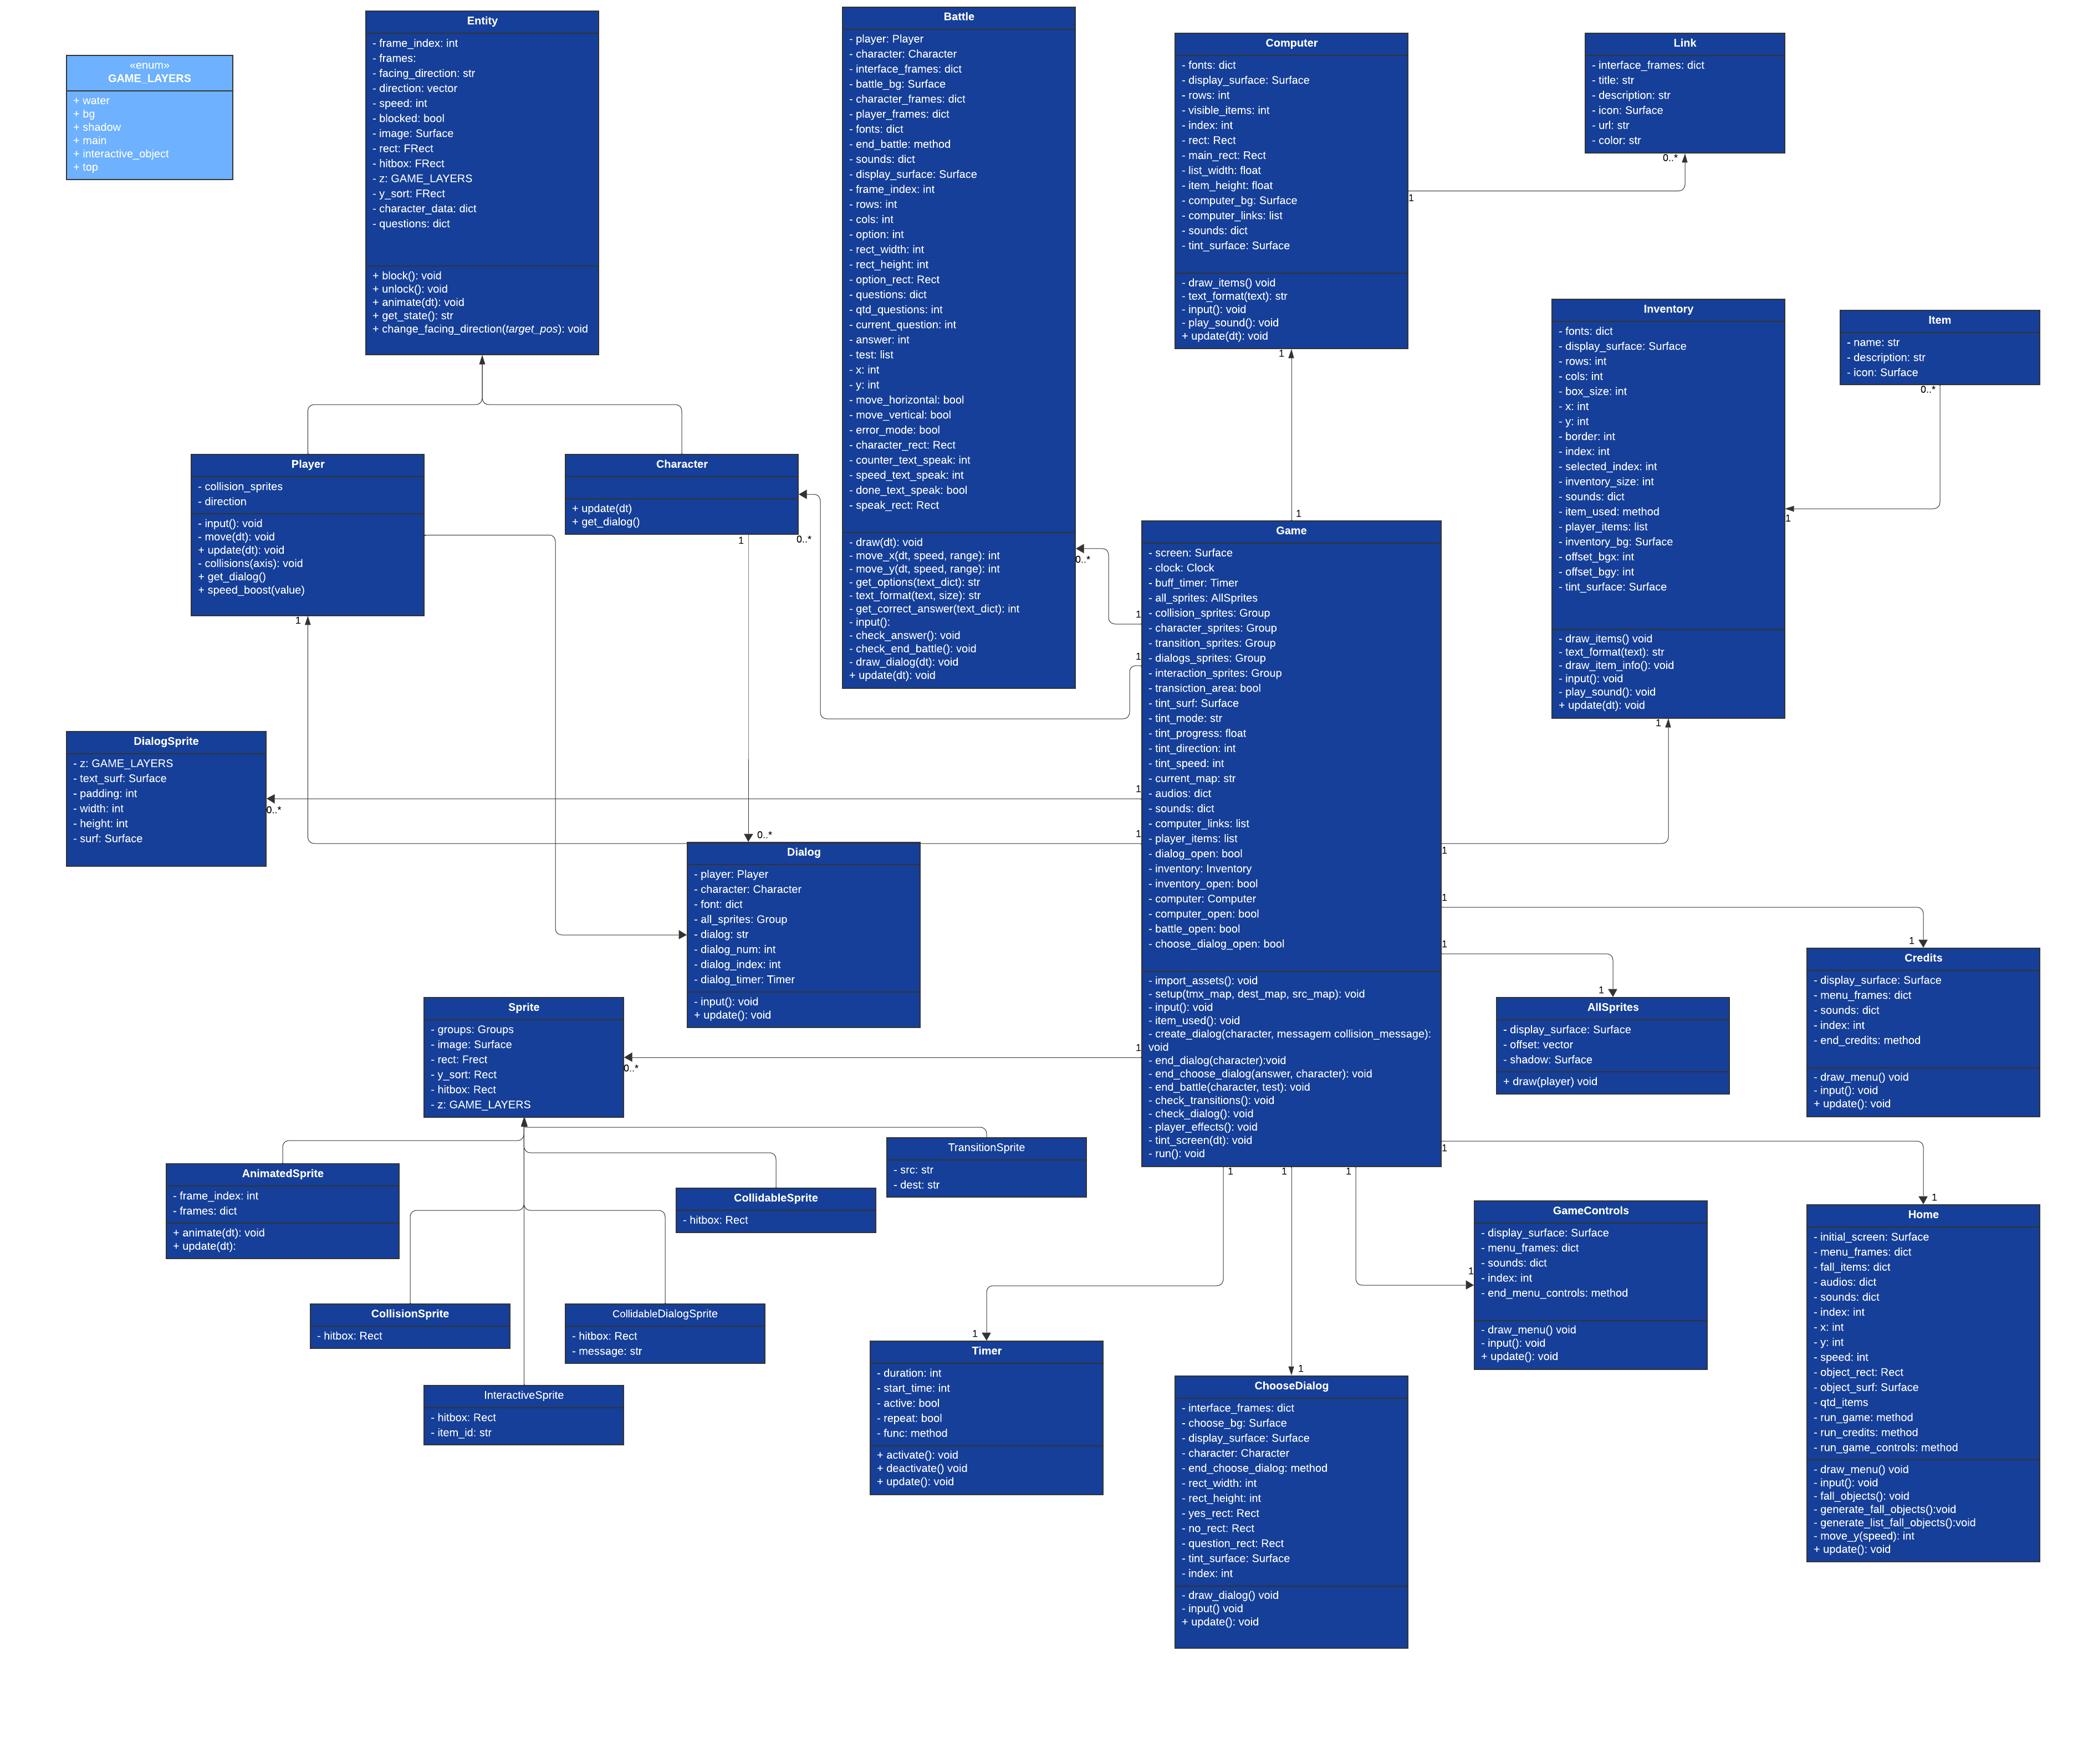
\includegraphics[width=0.8\linewidth]{figuras/diagrama-de-classes-uml.png}
    \caption{Diagrama de Classes do Super Labes World}
    \label{fig:diagrama-de-classes-uml}
\end{figure}
\end{landscape}

As tabelas \ref{tbl-especificacao-classes-1} e \ref{tbl-especificacao-classes-2}  apresentam mais informações sobre as classes propostas no diagrama.

\begin{table}[h!]
	\caption{Tabela especificando as classes do Super Labes World.}
	\label{tbl-especificacao-classes-1}
	\centering
	\renewcommand{\arraystretch}{2}
	\begin{small}
		\begin{tabular}{ | p{35mm} | p{100mm} |}\hline \rowcolor{MidnightBlue}
			\centering{\textbf{Classe}} & \textbf{Descrição}  \\\hline		
			\centering{\textit{AllSprites}} & Classe que representa a câmera do jogo. \\\hline
			\centering{\textit{Entity}} & Classe Pai usada para representar os personagens do jogo. Contém informações comuns a todas as entidades do jogo como frames, \textit{hitbox} e métodos relacionados a animação.   \\\hline
			\centering{\textit{Player}} & Classe filha de \textit{Entity}, representa o personagem que o jogador controla. Nele configuram-se atributos inerentes ao jogador, como a movimentação, colisão.  \\\hline
			\centering{\textit{Character}} & Classe filha de \textit{Entity} usada para representar os NPC's (Non Playable Character) ''personagens não jogáveis'' do jogo. Sua principal característica é o método para obtenção de diálogo relativo ao personagem.\\\hline
			\centering{\textit{Battle}} & Classe que representa a batalha do jogo. Contém todas as informações que fazem parte da batalha do jogo, destacando \textit{questions}, um dicionário com as questões relativas ao personagem e \textit{test}, uma lista que mantém um vetor de 0 para respostas erradas e 1 para respostas corretas.\\\hline
			\centering{\textit{Computer}} & Classe que representa a tela de visualização do computador do jogo. Contém o atributo \textit{computer\_links} que mantém um \textit{array} de \textit{Items} que serão mostrados ao entrar nessa tela. \\\hline
			\centering{\textit{Link}} & Representa um \textit{Link} do \textit{Computer}. Mantém informações que são utilizadas na interface \textit{Computer}. Sendo elas título, descrição, url, cor e icon que deve ser uma imagem 108 x 108 \\\hline
			\centering{\textit{Game}} & Classe que representa o jogo. Essa classe  mantém o \textit{main loop} e é responsável por carregar e armazenar todos os \textit{assets} e capturar o \textit{input} do jogador. \\\hline
			\centering{\textit{Inventory}} & Classe para representação da interface de inventário do jogador. \\\hline
			\centering{Item} & Classe que representa um Item do \textit{Inventory}. Mantém as informações dos items como nome, descrição e ícone, o tamanho ícone, que deve ser 93 x 93 \\\hline
		\end{tabular}
	\end{small}
\end{table}

\begin{table}[h!]
	\caption{Tabela com a continuação da especificação de classes do Super Labes World.}
	\label{tbl-especificacao-classes-2}
	\centering
	\renewcommand{\arraystretch}{2}
	\begin{small}
		\begin{tabular}{ | p{35mm} | p{100mm} |}\hline \rowcolor{MidnightBlue}
			  \centering{\textbf{Classe}} & \textbf{Descrição}  \\\hline
			\centering{\textit{DialogSprite}} & Classe que representa o dialogo do jogo. Ela realiza a renderização do diálogo na tela. \\\hline
			\centering{\textit{CollisionSprite}} & Classe filha de \textit{Sprite}, representa um sprite que pode ser colidido. Sua singularidade é ter uma \textit{hitbox}\\\hline
			\centering{\textit{CollidableSprite}} & Classe filha de \textit{Sprite}, representa um sprite que pode ser colidido, similarmente a \textit{CollisionSprite} porém a área de colisão dos \textit{sprites} nessa classe é menor.  \\\hline
			\centering{\textit{InteractiveSprite}} & Classe filha de \textit{Sprite}, representa um sprite interativo. Contém uma variável \textit{item\_id} que pode ser programada para diversos propósitos a partir de uma interação do jogador. \\\hline
			\centering{\textit{CollidableDialogSprite}} & Classe que herda \textit{Sprite}, usada para representar um diálogo caso jogador colide com determinadas posições do mapa. Essa classe não tem uma imagem associada e mantém uma mensagem que é disparada em colisões. \\\hline
			\centering{\textit{AnimatedSprite}} & Classe filha de \textit{Sprite}. Representa os \textit{Sprites} que animados do jogo. mantém um \textit{array} de \textit{frames} \\\hline
			\centering{\textit{TransitionSprite}} & Classe que herda \textit{Sprite}, representam os \textit{sprites} que levam para outros mapas. Guardam informações de origem e destino para poder realizar as transições entre mapas. \\\hline
			\centering{\textit{ChooseDialog}} & Classe que representa a interface de escolha do jogador antes de entrar em uma batalha. \\\hline
			\centering{\textit{Dialog}} & Classe pai que representa todos os diálogos do jogo. \\\hline
			\centering{\textit{Sprite}} & Classe Pai usada para representar todos os sprites do jogo. Suas informações são imagem, posição e camada. \\\hline
			\centering{\textit{Timer}} & Classe que representa o tempo no jogo. Responsável por realizar os controles de tempo do jogo. \\\hline
			  % \centering{\textbf{Classe}} & \textbf{Descrição}  \\\hline
			\centering{\textit{Home}} & Classe que representa a interface do menu inicial. \\\hline
			\centering{\textit{GameControls}} & Classe que representa a interface de controles do jogo, que pode ser acessada a partir da tela inicial. \\\hline
			\centering{\textit{Credits}} & Classe que representa a interface da tela de créditos que apenas pode ser acessada a partir da tela inicial.\\\hline
		\end{tabular}
	\end{small}
\end{table}

\clearpage
\section{Conclusões do Capítulo}
\label{sec:conclusoes-do-capitulo-3}
Este capítulo apresentou diversos aspectos essenciais para o desenvolvimento do jogo proposto. Inicialmente, foi estabelecido um cenário que foi o motivador para criação desse trabalho, nele é fornecido uma descrição objetiva do contexto em que o jogo está inserido. Essa definição facilita a compreensão dos desafios e metas a serem atingidos. Com isso foi possível definir o escopo que esse trabalho se propõe a atingir, bem como a história do jogo, e as suas principais mecânicas, e com isso foi feito o levantamento de requisitos.  

Por fim, foi apresentado o diagrama de classes, que desempenha um papel essencial na definição da estrutura do sistema. Com esse diagrama, foram identificadas as classes que representam os elementos do sistema e as relações entre elas. Esse diagrama junto a tabela de especificação de classes ajudaram na representação visual e facilitaram a compreensão das entidades do sistema e suas interações, auxiliando no planejamento para a implementação do sistema.

